\begin{itemize}
\item A non-parametric approach, which does
not make any assumptions about the underlying joint probability density function.Instead, it directly uses the data sample to estimate the density. Therefore, KNN could and probably should be one of the first choices for a classification study when there is little or no prior knowledge about the distribution data.
\item KNN is also a lazy algorithm .No Training ! Lack of generalization means that KNN keeps all the training data. To be more exact, all (or most) the training data is needed during the testing phase.
\item So, the predicted class for point x equation is given below where Ki is the neighbours of x.
\begin{figure}[H]
\centerline{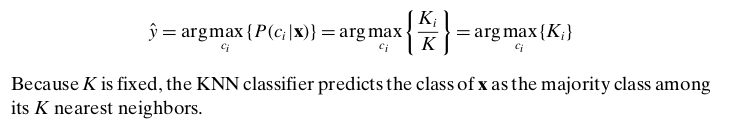
\includegraphics[width=1.2\textwidth]{Figures/knn.png}}
\caption{\label{fig:figure17}KNN Predicted Class Equation}
\end{figure}
\item KNN needs parameter tuning on the K which is the number of neighbors used to vote for the label and the distance function used to find the closest sample(s).
\item NEVER use the test set for the purpose of tweaking hyper parameters.\\For measuring the generalization of your classifier, Use the test set once at end.Use Validation sets for Hyper parameter Tuning.
\item Cross Validation for Classifier Tuning: 5-fold cross-validation run for the parameter k. For each value of k we train on 4 folds and evaluate on the 5th. For each k we receive 5 accuracies on the validation fold.\\
If we used more than 5 folds, we might expect to see a smoother (i.e. less noisy) curve.
\end{itemize}